\documentclass[fleqn,10pt]{wlscirep}
\usepackage[T1]{fontenc}
\usepackage[utf8]{inputenc}
\usepackage{lmodern}
\usepackage{graphicx}
\usepackage{booktabs}
\usepackage{placeins}
\usepackage{amsmath}
\usepackage{amssymb}
\usepackage{hyperref}
\hypersetup{
    colorlinks=true,
    linkcolor=blue,
    citecolor=blue,
    urlcolor=blue
}

\title{A Preliminary Study of ConvMixer in the Audio Domain Using Mel-Spectrogram Representation for Lightweight Speech Command Recognition}
\date{}

\author[1]{Ba-Tuan-Anh Chu}
\author[1]{Minh-An Luong}
\author[1]{Minh-Hoang Le}
\author[1,*]{Cong-Phuong Nguyen}
\author[1,*]{Thanh-Huong Nguyen}

\affil[1]{School of Electrical and Electronic Engineering, Hanoi University of Science and Technology, Hanoi, Vietnam}

\affil[*]{Corresponding authors: phuong.nguyencong@hust.edu.vn, huong.nguyenthanh3@hust.edu.vn}

% ABSTRACT
\begin{abstract}

Audio classification is a fundamental task pivotal to intelligent real-world systems, including voice control and environmental monitoring. However, conventional Convolutional Neural Networks (CNNs) often suffer from large parameter redundancy and limited generalization capability, whereas modern Transformer-based architectures typically necessitate significant computational overhead.
In this study, we present an empirical investigation of the ConvMixer architecture—a simple yet powerful model originally developed for computer vision—for audio classification using the Mel-spectrogram representation.
To our knowledge, this work represents an early and systematic effort to adapt ConvMixer to the audio domain, bridging vision-inspired patch-based design and efficient speech understanding.
The proposed framework incorporates a robust signal processing pipeline (denoising, WebRTC VAD, normalization) to generate fixed-size (128×32) Mel-spectrogram inputs. The ConvMixer model was configured with 8 deep blocks and 256 channels, utilizing approximately 0.7 million parameters.
On a Vietnamese speech command dataset of 1,853 samples and 13 classes, the ConvMixer-256/8 configuration achieved strong representative single-run performance (test accuracy 97.42\%, macro/weighted F1-score 0.97). To improve fairness and statistical reliability, we further define a controlled benchmark protocol in which ConvMixer-256/8, ResNet-18, MobileNetV2, EfficientNet, and AST (tiny configuration) are trained under the same preprocessing, augmentation, split policy, and training budget, and evaluated across five random seeds (42--46) using mean$\pm$std reporting. Under this controlled five-seed setting, ConvMixer-256/8 reached 97.63$\pm$0.59 test accuracy, with macro-F1 0.9761$\pm$0.0059 and weighted-F1 0.9763$\pm$0.0059, while using only 0.72M parameters.
Overall, these results and the revised protocol indicate that a purely convolutional patch-based architecture is a parameter-efficient and practical alternative for real-time speech command recognition, with clear potential for embedded and edge-AI deployment.

\end{abstract}


\begin{document}

\flushbottom

\maketitle
% SECTIONS
\section*{Introduction}

Recent advances in patch-based deep architectures have reshaped both vision and audio understanding, yet their adaptation to low-resource speech environments remains underexplored.
Audio classification is a core and rapidly evolving research field, fundamentally significant for constructing practical intelligent systems.
Typical applications include acoustic event detection, acoustic scene analysis, machinery fault diagnosis, and particularly speech command recognition.
In smart home or Internet of Things (IoT) systems, the ability to accurately and swiftly recognize speech commands is a prerequisite for ensuring optimal user experience.
Beyond that, lightweight and energy-efficient speech understanding models are increasingly essential for embedded AI, edge-AI, and low-power devices, where computational resources and latency are critical constraints \cite{lin2018edgespeechnetshighlyefficientdeep,howard2019searchingmobilenetv3,Wong2020TinySpeechAC}.
This practical demand highlights the importance of developing compact and efficient neural architectures for real-time speech command recognition \cite{9606720}.

A prevalent method in audio classification involves converting the raw signal into an information-rich two-dimensional representation, such as the Mel-spectrogram, which simulates how human hearing perceives frequencies.
This Mel-spectrogram representation is subsequently processed by deep learning models to learn temporal–spectral patterns.

For many years, traditional Convolutional Neural Networks (CNNs), such as ResNet, dominated computer vision and audio classification tasks due to their ability to exploit the locality and adjacency properties of spectral data \cite{Wightman2021ResNet}.
However, these CNN architectures often grapple with large parameter counts and occasionally encounter constraints in effective generalization.
More recently, Transformer-based models, notably the Vision Transformer (ViT), have demonstrated superior performance across various vision tasks \cite{dosovitskiy2020image}.
The Transformer leverages the self-attention mechanism to capture long-range global information \cite{zhu2023multiscaleaudiospectrogramtransformer,gong2021astaudiospectrogramtransformer,Koutini_2022}.
Despite their potency, ViT introduces a computational bottleneck: if self-attention were applied naively at the per-pixel level, the cost would scale quadratically with the image size, necessitating the division of the image into multiple “patches” (patch embeddings) before processing.
Similarly, other isotropic architectures like MLP-Mixer also operate by processing input patches \cite{Tolstikhin2021MLPMixer,liu2022convnet2020s,mehta2022mobilevitlightweightgeneralpurposemobilefriendly}.
This naturally poses a fundamental question: does the high performance of these newer architectures stem from the intrinsic power of the Transformer/MLP design, or is it, at least partially, due to the utilization of the patch-based representation?

To address this fundamental question and seek a more resource-efficient architecture, we focus on ConvMixer \cite{trockman2022patchesneed}.
ConvMixer is an extremely simple model, grounded in the core philosophy of separating spatial mixing and channel mixing, similar in principle to ViT \cite{dosovitskiy2020image} and MLP-Mixer \cite{Tolstikhin2021MLPMixer}.
The critical distinction is that ConvMixer performs all these mixing steps solely using standard convolutions.
This includes depthwise convolution for spatial mixing (often using a large kernel size, e.g., 9×9) and 1×1 pointwise convolution for channel mixing.
By inheriting the convolutional inductive bias—which is highly effective for image tasks—ConvMixer has demonstrated competitive accuracy against ViT, MLP-Mixer, and ResNet, often with fewer parameters and training resources \cite{trockman2022patchesneed}.
This architecture is uniquely suited to test the hypothesis that the utilization of a patch representation and an isotropic architecture is a critical factor driving the high performance of contemporary deep learning models.

Within the audio classification context, while Transformer-based models (such as the Audio Spectrogram Transformer—AST) have achieved remarkable results by leveraging large-scale pre-training knowledge (e.g., from ImageNet) \cite{Gong2021AST, Deng2009ImageNet}, they typically still face high complexity.
Crucially, the application and evaluation of the ConvMixer architecture—a simple, parameter-efficient, and effective patch-based convolutional model—within the audio domain, particularly for recognizing Vietnamese speech commands, remains a significant research gap.
This study aims to propose and rigorously evaluate the effectiveness of the ConvMixer architecture for the classification of Vietnamese speech commands.

To the best of our knowledge, this study is among the first systematic efforts to extend the ConvMixer architecture from computer vision to the audio domain.
Specifically, we pioneer its application to Mel-spectrogram-based Vietnamese speech command classification,
bridging a clear research gap and demonstrating that a purely convolutional patch-based approach can effectively capture temporal–spectral information without relying on self-attention mechanisms.
This novelty positions ConvMixer as a promising new direction for lightweight, efficient, and deployable speech understanding models.

The main contributions are four-fold: First, we propose a comprehensive audio processing pipeline incorporating advanced signal preprocessing (denoising, WebRTC VAD, and amplitude normalization) to ensure optimal input quality \cite{WebRTCVAD}, followed by the extraction of fixed-size Mel-spectrogram features with dimensions of 128×32.
Second, we implement and train a compact ConvMixer model (8 blocks, 256 channels, and approximately 0.7 million parameters) on the 13-class Vietnamese speech command dataset with targeted data augmentation.
Third, we establish a controlled comparison protocol on the same dataset and training budget for ConvMixer-256/8, ResNet-18, MobileNetV2, EfficientNet, and AST (tiny configuration), enabling a fairer model-level assessment under identical preprocessing and feature settings.
Fourth, we strengthen statistical reliability by evaluating all compared models over five random seeds (42--46) and reporting mean$\pm$std metrics, while retaining detailed class-wise error analysis to explain model behavior.
Overall, this revised study positions ConvMixer as a computationally efficient and competitive patch-based convolutional alternative for Vietnamese speech command recognition. Figure~\ref{fig:comparison} provides a conceptual comparison between generic patch-based architectures (on the left) and the proposed ConvMixer adaptation for the audio domain (on the right), highlighting the key architectural differences. In particular, the figure illustrates how ConvMixer replaces self-attention and MLP-based token mixing with purely convolutional spatial–channel mixing, thereby retaining the benefits of patch-based representation while reducing model complexity.


\begin{figure}[htbp]
\centering
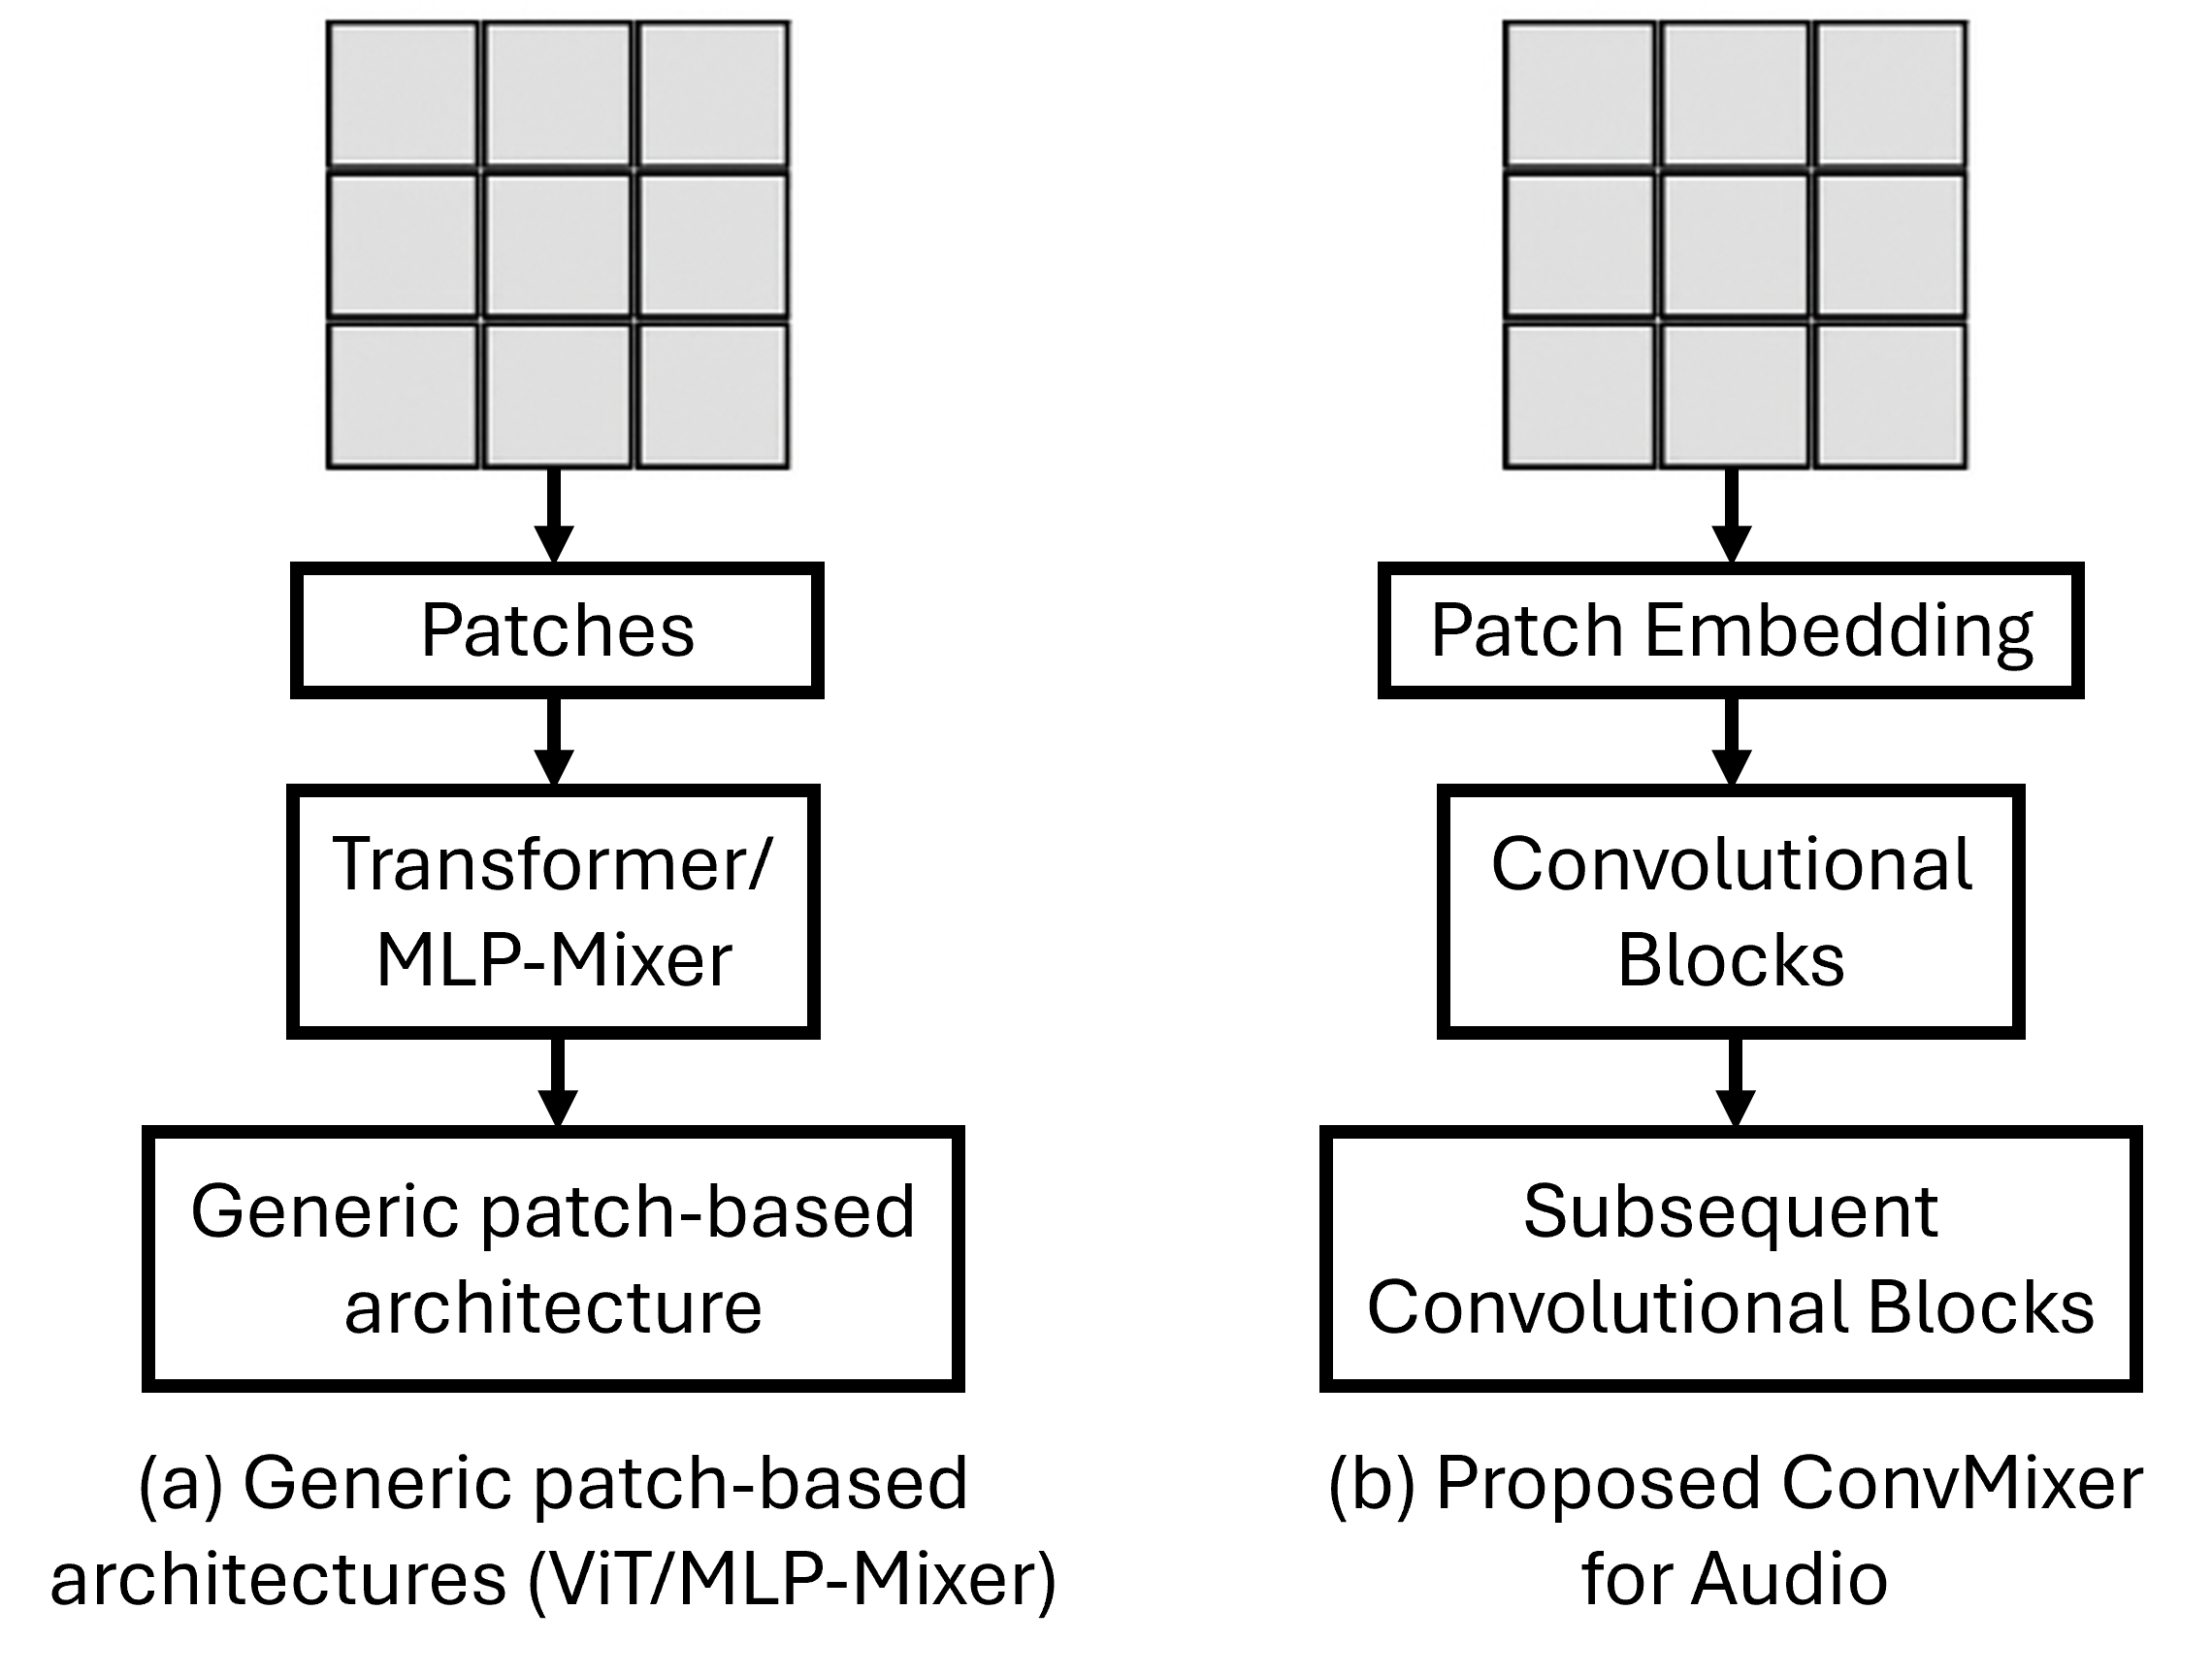
\includegraphics[width=0.55\linewidth]{imgs/Convmixer-comparison.png}
\caption{\label{fig:comparison}Conceptual comparison diagram of audio patch-based models.}
\end{figure}

The structure of this paper is organized as follows: Section 2 reviews related works, focusing on the evolution from CNNs to Transformer architectures and ConvMixer.
Section 3 details the proposed methodology, encompassing data preprocessing steps, Mel-spectrogram feature extraction, and the ConvMixer architecture.
Section 4 presents the experiments, quantitative results, and performance analysis.
Section 5 discusses the key findings, compares the model against foundational architectures, and addresses the study's limitations.
Finally, Section 6 provides the conclusion and outlines directions for future work.

\section*{Related Works}

This review of related works presents the developmental context of audio classification methodologies, spanning from traditional feature extraction techniques to modern deep learning models, including architectures based on Convolution and Self-Attention. This context serves to position the necessity for an efficient, simple, and patch-based architecture such as ConvMixer within the field of audio classification.
In the revised version, we also reorganize the reference narrative to emphasize peer-reviewed and methodologically relevant studies, while keeping citation formatting consistent throughout the manuscript.

\subsection*{Traditional Audio Classification Approaches}

In the initial stages, audio classification relied predominantly on manually extracting features from the raw signal. Popular features included Mel-Frequency Cepstral Coefficients (MFCC), Spectrograms, and Chroma features. The Mel-spectrogram, a time-frequency representation based on the Mel scale simulating human auditory perception, has established itself as the standard benchmark in speech and music processing \cite{Stevens1937MelScale}. After feature extraction, classical machine learning models, typically Support Vector Machines (SVM) or Random Forests (RF), were employed for classification. Although these methods provided a solid foundation, their performance was inherently limited by the representational capacity of manual features and their inability to fully exploit complex relationships within large-scale audio data.

\subsection*{Deep Learning Models Based on CNN and Transformer}

The emergence of deep learning revolutionized the field of audio classification. Convolutional Neural Networks (CNN) rapidly became the dominant architecture due to their capacity to exploit the locality and translation invariance of audio spectral data, which are typically treated as 2D images. Several approaches have been proposed, including architectures such as ResNet, EfficientNet, and PANN (Pretrained Audio Neural Networks) \cite{Wightman2021ResNet, Kong2020PANNs}, which were developed to enhance the capture of semantic information on the audio spectrum, achieving high performance in tasks like speech command recognition and acoustic event detection. Previous studies have shown that deep CNN models, however, often require a large number of parameters and sometimes struggle to effectively model long-range dependencies across the spectrogram.

To address this limitation, Transformer-based architectures were introduced, initially in Computer Vision (CV) with the Vision Transformer (ViT) \cite{dosovitskiy2020image}. ViT demonstrated superior performance compared to traditional CNNs, especially when trained on large-scale datasets. The key to the Transformer's success lies in its use of the self-attention mechanism to capture global information. However, because the computational cost of self-attention scales quadratically with the number of pixels, ViT must convert the input image into "patches" (patch embeddings) before processing. The Audio Spectrogram Transformer (AST) is the audio domain adaptation of ViT, achieving impressive results by leveraging pre-training knowledge, often from ImageNet and AudioSet \cite{Gong2021AST, Deng2009ImageNet, Gemmeke2017AudioSet}. Subsequently, a range of other "isotropic" architectures emerged, such as MLP-Mixer and ResMLP, seeking to understand the impact of patch-based processing and uniform network structure \cite{Tolstikhin2021MLPMixer, Touvron2021ResMLP}.

\subsection*{ConvMixer: Simple, Efficient, and Patch-Based}

The emergence of ViT and MLP-Mixer models prompted a fundamental inquiry regarding whether their superior performance stems from the intrinsic Transformer/MLP architecture or is at least partially attributable to the adoption of a patch-based representation \cite{dosovitskiy2020image, Tolstikhin2021MLPMixer}. ConvMixer was proposed as a minimalistic yet powerful model, operating directly on input patches while maintaining uniform size and resolution throughout the network, similar to ViT and MLP-Mixer \cite{trockman2022patchesneed}. Its key distinction is that all necessary mixing operations—spatial and channel mixing—are performed solely using standard convolutions. Specifically, ConvMixer uses large-kernel depthwise convolutions for spatial mixing and $1\times 1$ pointwise convolutions for channel mixing.

Despite its compact architecture (implementable in approximately six lines of PyTorch code) \cite{Paszke2019PyTorch, trockman2022patchesneed}, ConvMixer achieves competitive accuracy compared to ResNet, ViT, and MLP-Mixer when parameter counts are similar \cite{trockman2022patchesneed}. For example, experiments on CIFAR-10 show that ConvMixer can exceed 96\% accuracy with only 0.7 million parameters, demonstrating the data efficiency conferred by convolutional inductive bias \cite{trockman2022patchesneed}. While more complex patch-based models such as the Audio Spectrogram Transformer (AST) have been widely applied \cite{Gong2021AST}, the adaptation and empirical evaluation of ConvMixer in the audio domain—particularly for Vietnamese speech command recognition—has not been previously reported. 

To the best of our knowledge, this work constitutes an early empirical study that adapts and validates ConvMixer for Mel-spectrogram-based audio classification, highlighting its potential as a lightweight and resource-efficient alternative to deeper CNN and Transformer architectures in practical audio tasks.

In this revised manuscript, we position novelty in a constrained and testable manner: the contribution is not the invention of a new backbone, but a controlled adaptation-and-evaluation study that transfers ConvMixer to Vietnamese speech command recognition with a unified preprocessing pipeline, matched training protocol across baselines, and multi-seed statistical reporting.
This scope is intentionally narrower than large-scale pretraining studies, but it provides clearer evidence on model behavior in low-resource, deployment-oriented settings.

\begin{table}[h!]
\centering
\caption{Comparison of representative architectures in audio and vision-audio classification tasks.}
\resizebox{\linewidth}{!}{
\begin{tabular}{lcccc}
\hline
\textbf{Model} & \textbf{Params (M)} & \textbf{GFLOPs} & \textbf{Accuracy (\%)} & \textbf{Dataset} \\
\hline
ResNet-18 (CNN) & 11.7 & 1.8 & 94.5 & Speech Commands v2 \\
ViT-Base (Transformer) & 86.0 & 17.6 & 97.0 & AudioSet / ImageNet \\
AST (Audio Spectrogram Transformer) \cite{Gong2021AST} & 88.0 & 17.0 & 98.1 & AudioSet \\
AclNet (CNN) \cite{Huang2018AclNet} & 0.16 & 0.05 & 81.8 & ESC-50 \\
PIPMN (MLP) \cite{Chen2022PIPMN} & 1.0 & 0.2 & 96.0 & UrbanSound8K \\
VATT (Transformer) \cite{Akbari2021VATT} & 38.7 & 14.5 & 97.5 & AudioSet \\
\textbf{ConvMixer-256/8 (ours)} & \textbf{0.72} & \textbf{0.3} & \textbf{97.14} & Vietnamese Speech Commands \\
\hline
\end{tabular}}
\label{tab:comparison_models}
\end{table}

{\footnotesize
Note: Accuracy values are reported from the original papers and are not directly comparable due to differences in datasets. ConvMixer results are obtained on Vietnamese Speech Commands. To ensure fairer assessment, this study additionally reports controlled same-dataset comparisons across multiple lightweight models in the Results section.
}

\vspace{1pt}

Building on this perspective, the next section describes the proposed methodology, including audio preprocessing, Mel-spectrogram feature extraction, and the ConvMixer-based classification framework.

\section*{Methods}

This study proposes a comprehensive and systematic procedure for classifying Vietnamese speech commands using the ConvMixer architecture \cite{trockman2022patchesneed} in the audio domain. The focus lies in optimizing both input feature quality and architectural efficiency, while establishing a controlled and statistically robust comparison protocol across multiple lightweight models.

Figure~\ref{fig:novelty} illustrates the conceptual novelty of adapting the ConvMixer architecture to the audio domain using Mel-spectrogram representations. As shown on the left, the input Mel-spectrogram encodes time–frequency energy patterns of speech signals, which are treated as a two-dimensional structure analogous to an image. The spectrogram is first partitioned into local patches, enabling patch-level feature abstraction while preserving the inherent temporal–spectral structure of audio signals.

\begin{figure}[htbp]

\centering

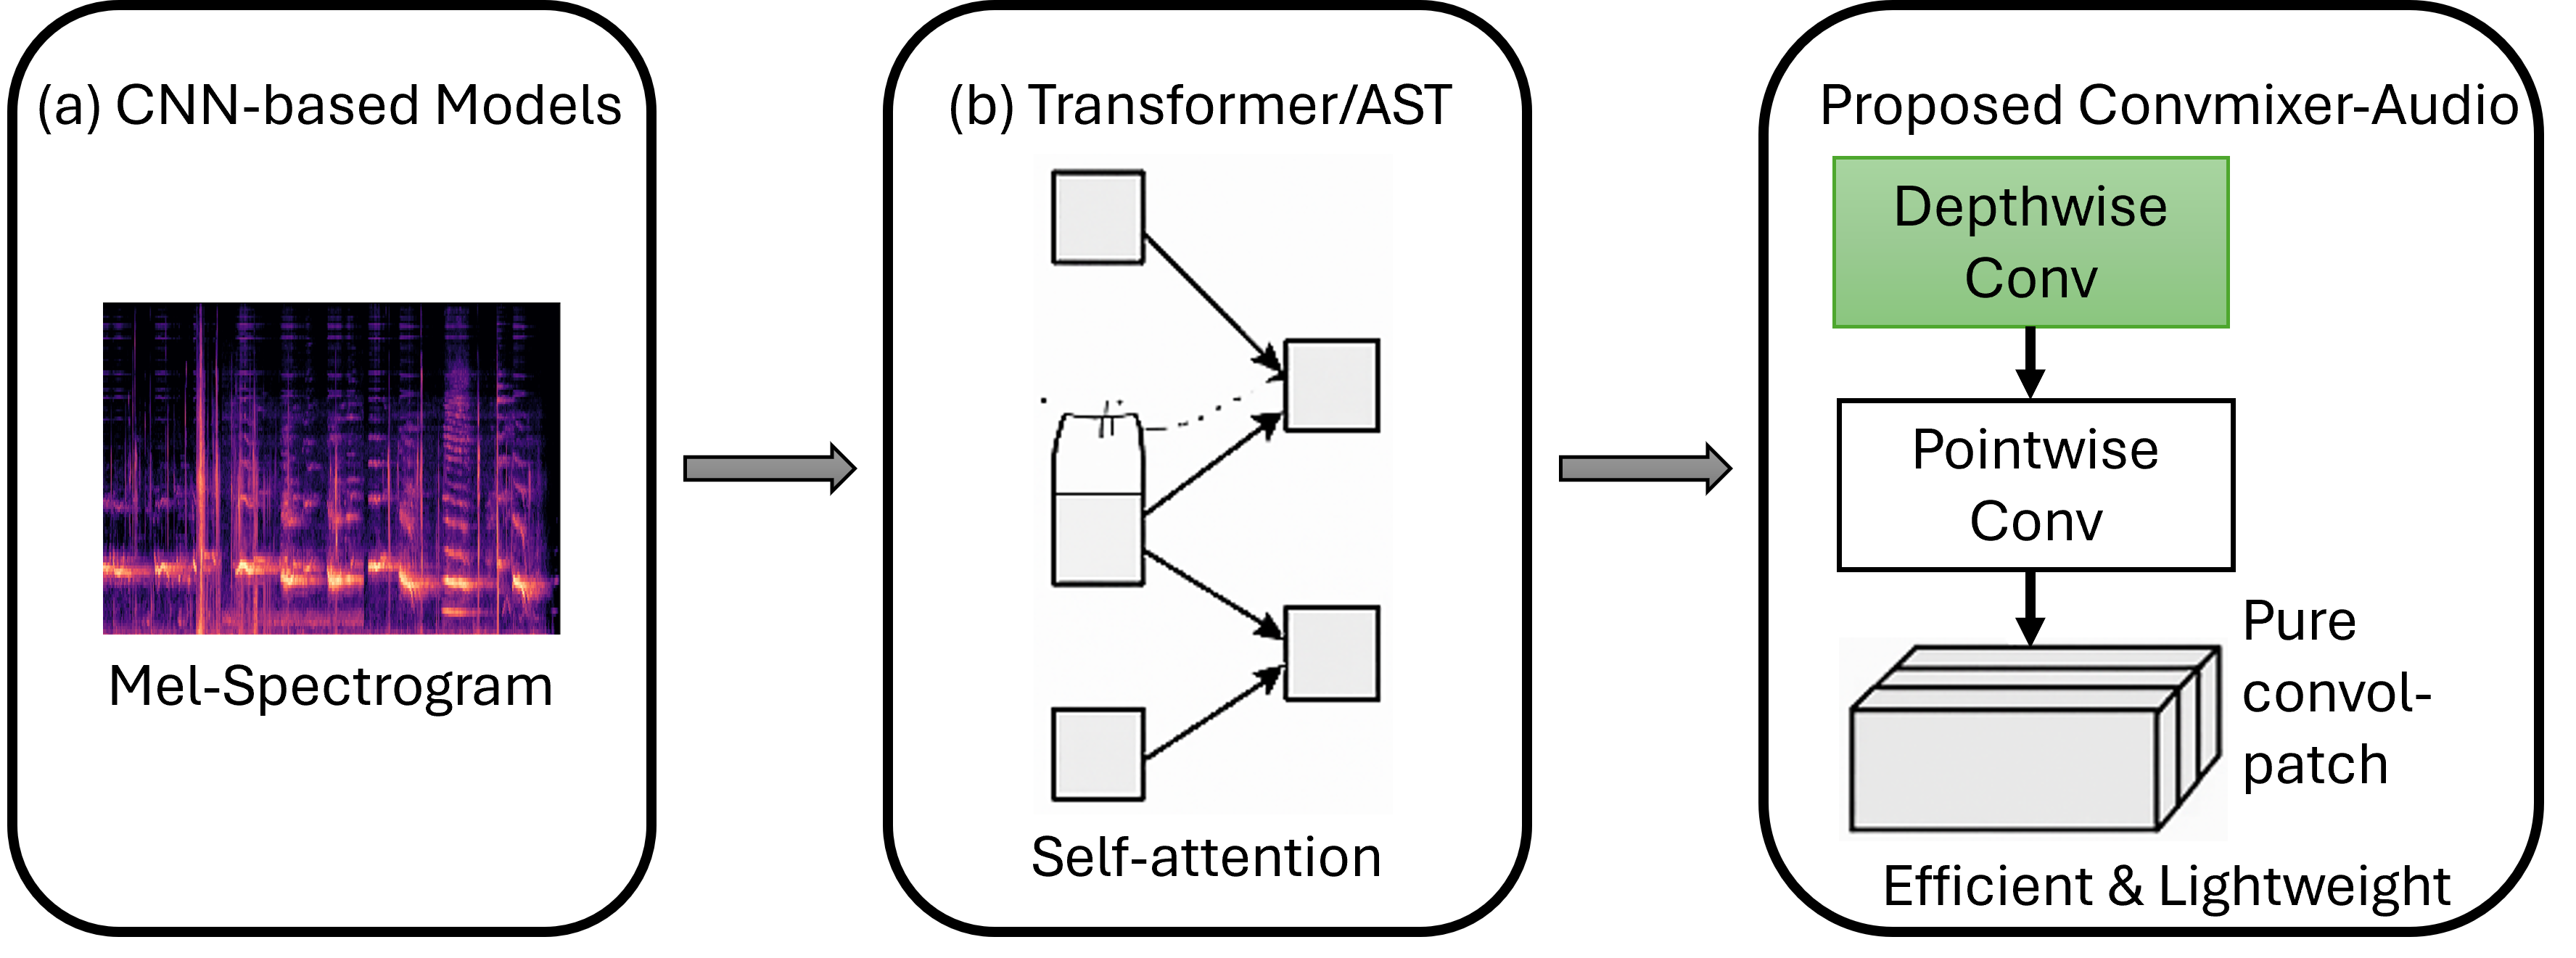
\includegraphics[width=0.8\linewidth]{imgs/Convmixer-novelty.png}

\caption{\label{fig:novelty}Conceptual diagram of ConvMixer audio novelty}

\end{figure}

Unlike attention-based or MLP-based patch models, the proposed ConvMixer-Audio framework performs feature mixing exclusively through convolutional operations. Specifically, depthwise convolution is employed to capture spatial relationships within each patch across the time–frequency plane, effectively modeling local and mid-range temporal–spectral dependencies. Subsequently, pointwise convolution enables channel-wise feature interaction, facilitating global feature integration across patches.

This convolution-only patch-based design eliminates the need for self-attention mechanisms while retaining the representational benefits of patch processing. As a result, ConvMixer achieves a favorable balance between expressive capacity and computational efficiency, highlighting its suitability for lightweight, deployable speech understanding systems in edge-AI and embedded environments.


\begin{figure}[htbp]

\centering

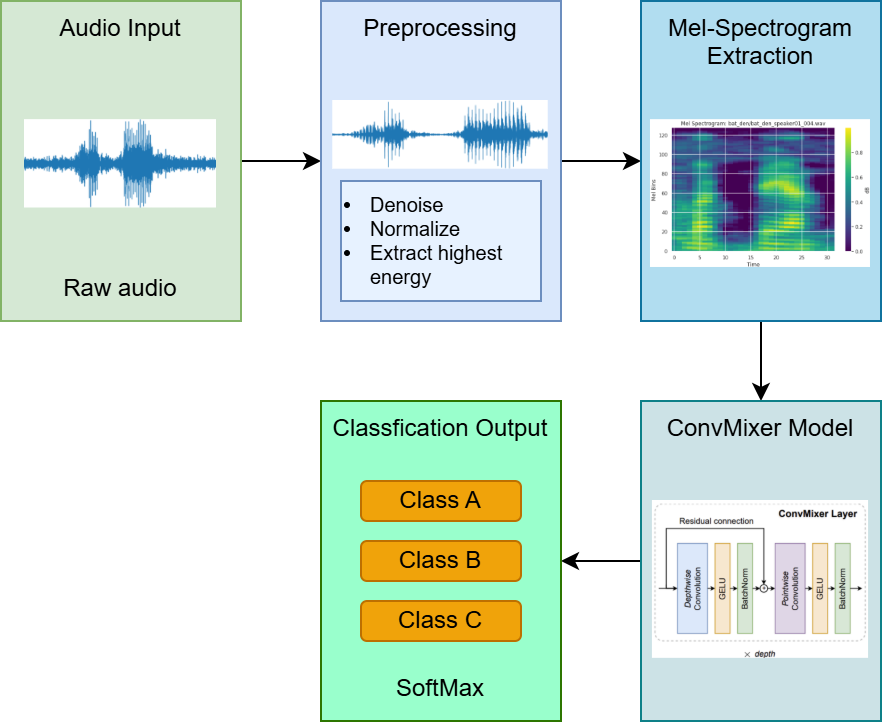
\includegraphics[width=0.8\linewidth]{imgs/fig1.png}

\caption{\label{fig:overview}Overview of the proposed audio classification framework. The pipeline includes raw audio input, preprocessing (denoising, normalization, and energy-based segmentation), Mel-spectrogram feature extraction, ConvMixer-based model training, and final classification using the Softmax layer}

\end{figure}



\subsection*{Audio Preprocessing}

A refined preprocessing pipeline was designed to produce standardized, noise-reduced, and energy-balanced one-second speech segments for Mel-spectrogram extraction. Compared with the baseline version, this workflow introduces two key enhancements—Voice Activity Detection (VAD) and a two-stage high-energy segment extraction—substantially improving the quality and consistency of speech features for lightweight ConvMixer models. Figure~\ref{fig:overview} presents an overview of the proposed end-to-end audio classification framework based on the ConvMixer architecture. The pipeline begins with raw audio input, which undergoes a dedicated preprocessing stage including denoising, amplitude normalization, and energy-based segmentation to ensure consistent and informative speech segments. These operations aim to suppress background noise, remove silence, and standardize signal amplitude, thereby improving the robustness of downstream feature extraction.

The pipeline begins by loading the raw recordings, converting them to mono, and resampling at 16~kHz to retain the 0–4~kHz speech band while reducing data size. Spectral noise reduction is then applied using subtraction or gating in the frequency domain to suppress background interference and enhance clarity.

Voice Activity Detection (VAD) is performed using Google’s WebRTC algorithm~\cite{WebRTCVAD}, which analyzes 30~ms frames and removes non-speech intervals. A sensitivity level of~2 offers a balanced trade-off between preserving speech and eliminating silence or background noise.

Next, a two-stage high-energy extraction ensures consistent and content-rich inputs. A 1.5-second sliding window (stride 0.3~s) first identifies the segment with the highest total energy, followed by a finer 1-second search (stride 20~ms) within that region to locate the most informative sub-segment. This hierarchical approach captures the most relevant portion of each utterance while standardizing duration.

Finally, peak normalization scales each waveform to a uniform amplitude, with the maximum absolute value set to~0.99 of the dynamic range and converted to 16-bit integer format. The resulting one-second segments are noise-suppressed, amplitude-normalized, and rich in speech information, providing stable and high-quality inputs for Mel-spectrogram feature extraction. Figure~\ref{fig:preprocessing} illustrates the complete preprocessing flow.

\begin{figure}[htbp]
\centering
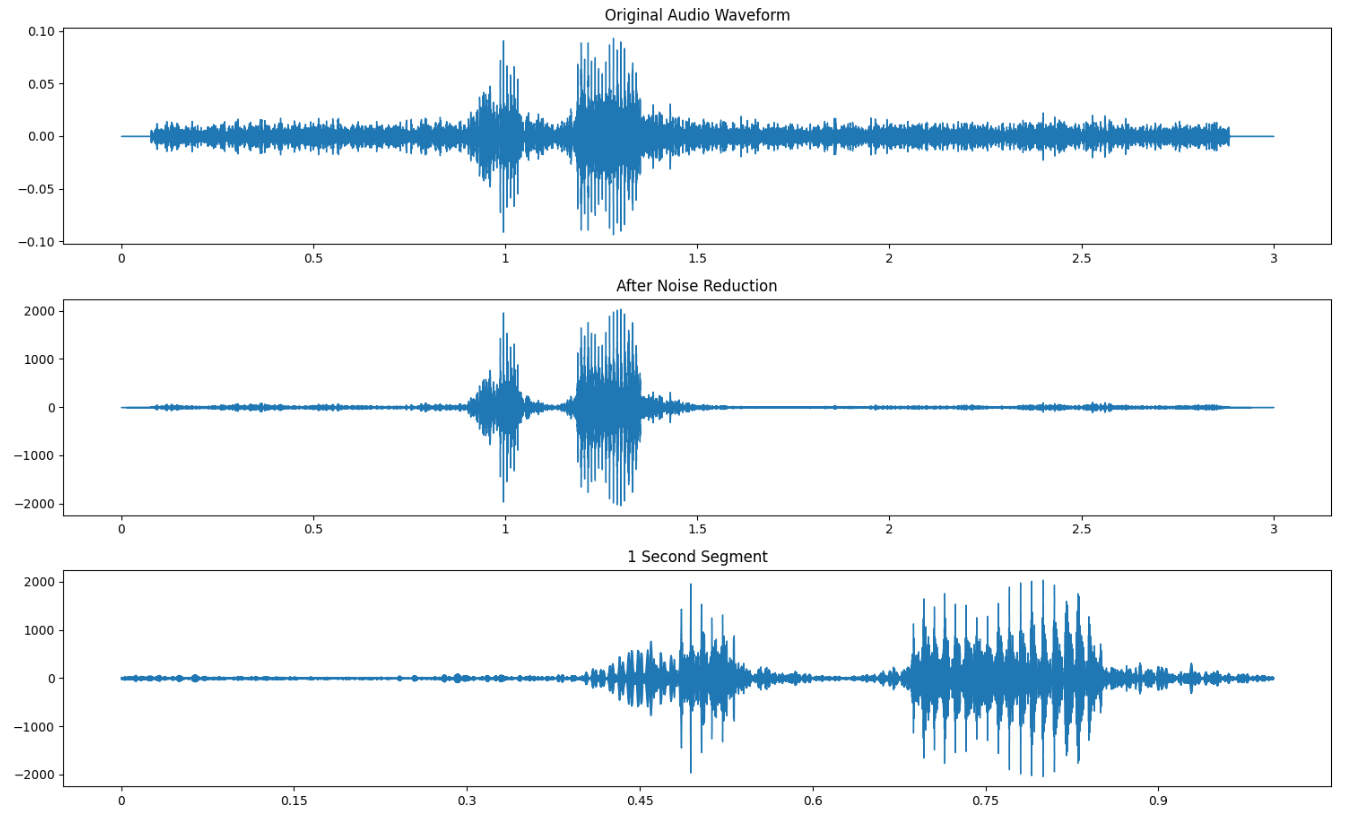
\includegraphics[width=0.75\linewidth]{imgs/fig2.png}
\caption{\label{fig:preprocessing}Overview of the audio preprocessing pipeline. The raw waveform undergoes denoising, voice activity detection (VAD), normalization, and segmentation into 1-second clips before feature extraction.}
\end{figure}



\subsection*{Mel-spectrogram Feature Extraction}

The input feature for the ConvMixer model is the Mel-spectrogram, a 2D representation aligned with human auditory perception on the Mel scale~\cite{Stevens1937MelScale}. The extraction parameters were configured as follows\cite{mcfee2015,Park_2019}:

\begin{itemize}

\item \textbf{STFT parameters:}  
The window size ($n\_fft = 2048$) and hop length ($hop\_length = 128$) were selected for fine-grained temporal resolution. With a 16~kHz sampling rate, each frame corresponds to 0.008~s, suitable for short speech events.  
The Short-Time Fourier Transform (STFT) converts overlapping time-domain frames $x[n]$ into their frequency components using a Hann window:
\[
X(f, t) = \sum_{n=0}^{N-1} x[n] w[n - t \cdot hop\_length] e^{-j 2 \pi f n / N}.
\]

\item \textbf{Mel parameters:}  
A 128-band Mel filter bank was applied, covering 20–8000~Hz (the Nyquist range). The Mel scale mapping is:
\[
m = 2595 \log_{10}\left(1 + \frac{f}{700}\right),
\]
which provides higher resolution at perceptually important low frequencies.

\item \textbf{Conversion and normalization:}  
The power spectrum was computed as $P(f, t) = |X(f, t)|^2$ and filtered by triangular Mel filters $W(m, f)$ to produce the Mel power spectrum:
\[
P_{\text{Mel}}(m, t) = \sum_f W(m, f) \cdot P(f, t).
\]
It was then converted to the logarithmic scale:
\[
\text{Mel-spectrogram (dB)} = 10 \log_{10}\left(\frac{P_{\text{Mel}}}{P_{\text{ref}}} + \epsilon\right),
\]
with $\epsilon = 10^{-10}$ ensuring numerical stability.  
Finally, Min–Max normalization was applied:
\[
X_{\text{norm}} = \frac{X - X_{\min}}{X_{\max} - X_{\min}},
\]
producing values in the $[0, 1]$ range for consistent model input.

\end{itemize}

The resulting Mel-spectrograms were resized to a fixed dimension of $128 \times 32$ (128 Mel bins, 32 time frames) using bilinear interpolation and stored as \texttt{.npy} files for model training. All feature extraction steps (STFT computation, Mel filtering, log compression, and normalization) were implemented using Librosa and Torchaudio to ensure consistent and reproducible spectrogram generation across experiments\cite{mcfee2015,Park_2019}. Additionally, SpecAugment-based masking operations were incorporated as part of the data augmentation pipeline\cite{Park_2019}.

\begin{figure}[htbp]
\centering
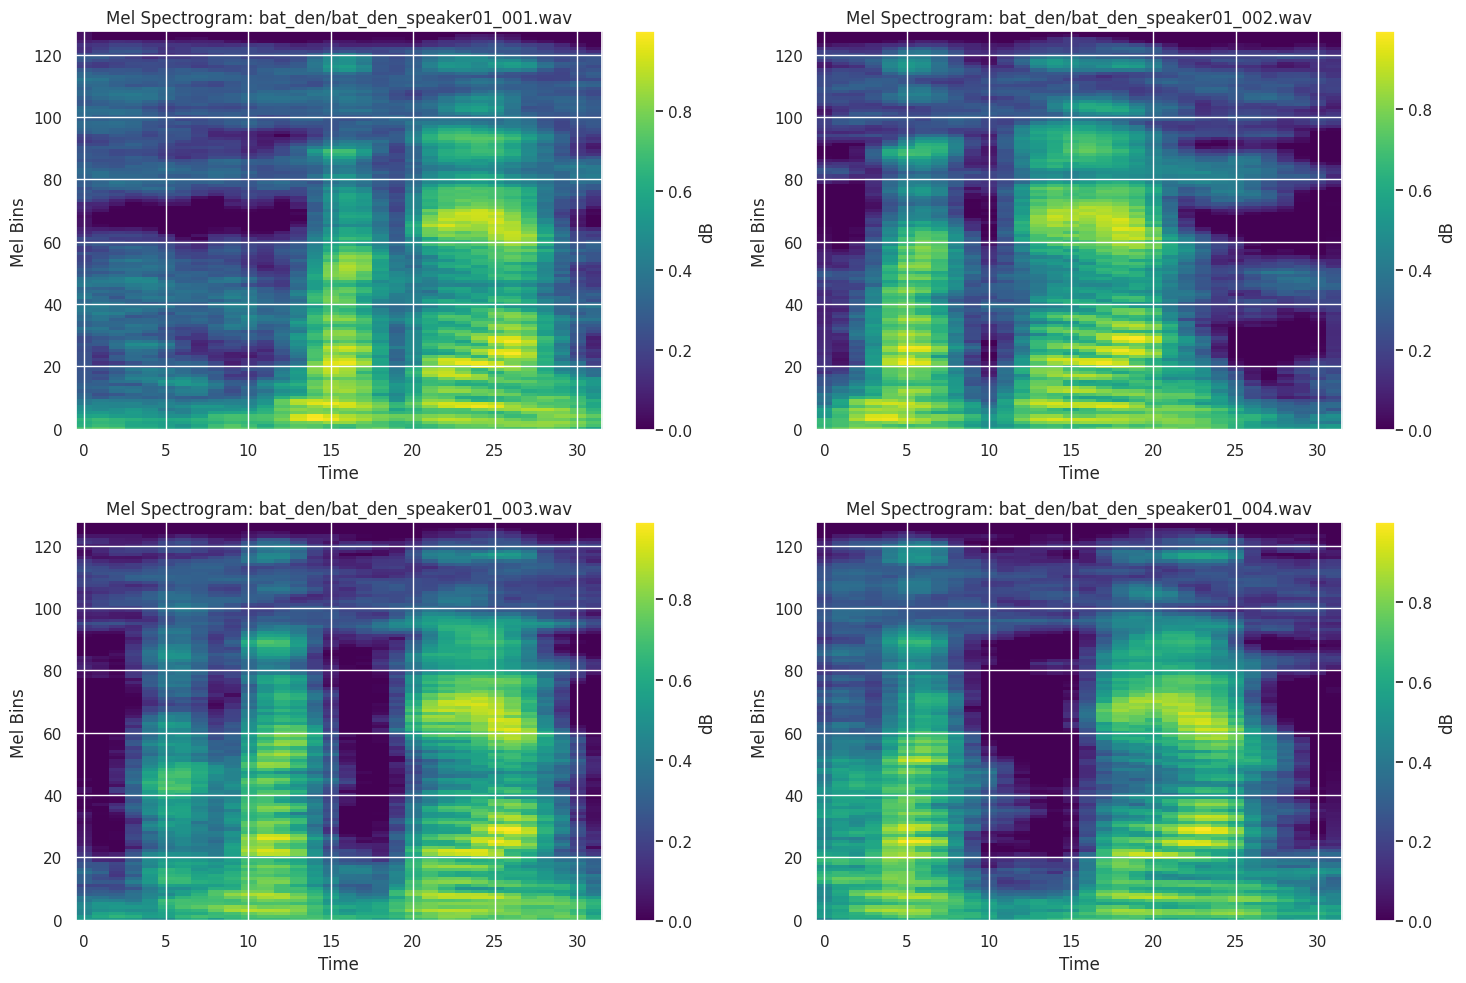
\includegraphics[width=0.75\linewidth]{imgs/fig3.png}
\caption{\label{fig:melspec}Example Mel-spectrograms of four “bat\_den” (turn-on light) samples after preprocessing. The time–frequency patterns highlight energy concentration across specific bands.}
\end{figure}


\subsection*{Data Augmentation}

To enhance model robustness and mitigate overfitting on the relatively small dataset (1,853 samples), state-of-the-art data augmentation techniques were applied only to the training set. Time Masking was applied with a 50\% probability, randomly covering up to 10\% of the time dimension. Frequency Masking was also applied with a 50\% probability, randomly covering up to 10\% of the Mel bins. Furthermore, Time Stretching was used with a 50\% probability, altering the playback speed between 80\% and 120\% of the original duration via linear interpolation, before resizing the feature back to the original dimensions of 128 × 32 \cite{Cubuk2020RandAugment, Zhang2017Mixup, Yun2019CutMix, Zhong2020RandomErasing}.

\subsection*{ConvMixer Architecture}

The ConvMixer architecture was employed for its simplicity and parameter efficiency, operating on a patch representation similar to ViT and MLP-Mixer but utilizing only standard convolutions for both spatial and channel mixing \cite{trockman2022patchesneed, dosovitskiy2020image, Tolstikhin2021MLPMixer}. Unlike attention-based models, ConvMixer preserves convolutional inductive biases such as spatial locality and translation equivariance while retaining the patch-based abstraction of vision transformers.

The implemented model follows the ConvMixer-256/8 configuration, where the hidden dimension ($dim = 256$) and depth ($depth = 8$) define the number of feature channels and repeated mixing blocks, respectively. This setting results in approximately 0.72 million trainable parameters, striking a balance between expressive capacity and computational efficiency. Preliminary ablation trials with smaller (ConvMixer-128/8) and deeper variants (ConvMixer-256/12) revealed that ConvMixer-256/8 offered the best trade-off between accuracy and model complexity, avoiding overfitting while maintaining fast convergence.

\begin{itemize}
\item \textbf{Patch Embedding:} The single-channel input ($1 \times 128 \times 32$) is transformed into 256-channel patch embeddings through a convolutional stem:
\begin{equation*}
X_0 = \text{GELU}(\text{BN}(\text{Conv}_{7\times7,\,stride=7}(X))),
\end{equation*}
where $\text{Conv}_{7\times7}$ extracts local structures within each patch while downsampling the feature map by a factor of 7 in both dimensions.

\item \textbf{ConvMixer Blocks:} Each of the $L=8$ repeated blocks performs spatial and channel mixing:
\begin{align*}
Z' &= X + \text{GELU}(\text{BN}(\text{DWConv}_{9\times9}(X))), \\
X' &= \text{GELU}(\text{BN}(\text{Conv}_{1\times1}(Z'))),
\end{align*}
where $\text{DWConv}$ denotes depthwise convolution (grouped by $dim$). The residual connection maintains gradient stability and preserves low-level information, while the $(1\times1)$ convolution enables full cross-channel interaction analogous to MLP mixing layers.

\item \textbf{Output Head:} The final feature map is globally aggregated via adaptive average pooling:
\begin{equation*}
y = \text{Linear}(\text{Flatten}(\text{AvgPool}(X_L))),
\end{equation*}
producing 13 class logits corresponding to the target categories.
\end{itemize}

Overall, the ConvMixer architecture can be summarized as a hierarchical composition:
\begin{equation*}
f(X) = \text{Linear}(\text{AvgPool}(\text{MixBlock}_L(\dots \text{MixBlock}_1(\text{PatchEmbed}(X))))),
\end{equation*}
where $\text{MixBlock}_i$ alternates between spatial and channel mixing. This compact yet expressive design retains the representational power of deep convolutional models while maintaining computational efficiency, making it well-suited for real-time and embedded speech recognition tasks.


\subsection*{Training Configuration}

\subsubsection*{Dataset Split}
The dataset of 1,853 Vietnamese speech command samples was divided using a stratified split to maintain class balance across subsets: 75\% for training (1,385 samples), 15\% for validation (274 samples), and 10\% for testing (194 samples). Each subset preserves proportional representation of all 13 classes. This split policy was fixed and shared by all compared architectures.

\subsubsection*{Optimization Settings}
Training was performed using the Adam optimizer with an initial learning rate ($lr = 0.001$) and weight decay ($1 \times 10^{-4}$) for L2 regularization \cite{Loshchilov2018AdamW}. The batch size was set to 32, and the CrossEntropyLoss function was applied for multi-class classification.

\subsubsection*{Learning Rate Scheduling}
A $ReduceLROnPlateau$ scheduler was used to automatically adjust the learning rate, operating in \textit{‘max’} mode to monitor validation accuracy. The learning rate decayed by a factor of 0.2 if no improvement was observed for 3 consecutive epochs, with a minimum learning rate threshold of $1 \times 10^{-6}$.

\subsubsection*{Regularization and Early Stopping}
To prevent overfitting, Early Stopping was employed with a patience of 5 epochs and a minimum required improvement ($min\_delta = 0.02$) in validation accuracy. The maximum training duration was capped at 25 epochs, balancing computational efficiency and model stability.

\subsubsection*{Controlled Baseline Protocol}
To address fairness concerns in cross-model evaluation, we define a controlled benchmark in which ConvMixer-256/8, ResNet-18, MobileNetV2, EfficientNet, and AST (tiny configuration) are trained on exactly the same dataset split, with identical preprocessing, Mel-spectrogram extraction settings, augmentation strategy, optimizer family, early stopping policy, and epoch budget. This design isolates architectural effects and avoids confounding factors caused by inconsistent pipelines.

For the ResNet baseline, we adopt a standard ResNet-18 configuration adapted to spectrogram input by setting the first convolution to one input channel and replacing the classification head with a 13-class output layer.

For the transformer baseline, we use the official AST implementation (\url{https://github.com/YuanGongND/ast/}) with a tiny configuration (reduced embedding width and depth) \cite{Gong2021AST} so that training cost remains comparable to lightweight convolutional baselines while preserving the core patch-embedding and self-attention mechanism.

\subsubsection*{Multi-seed Statistical Evaluation}
To improve result reliability on a relatively small dataset, each model is trained with five random seeds: 42, 43, 44, 45, and 46. For each metric (Accuracy, macro-F1, weighted-F1, and loss), we report mean$\pm$std across seeds. We additionally compute a 95\% confidence interval for the mean when needed:
\[
\mathrm{CI}_{95\%} = \bar{x} \pm 1.96\frac{s}{\sqrt{n}}, \quad n=5.
\]
This protocol reduces dependence on a single random run and provides a more stable basis for model comparison.

\section*{Results}

This section presents the experimental outcomes under two complementary perspectives: (i) detailed ConvMixer behavior analysis, and (ii) controlled cross-model comparison under an identical training protocol with multi-seed reporting.

\subsection*{Dataset Setup}

The investigation was conducted using a Vietnamese speech command dataset comprising a total of 4,460 audio samples, classified into 13 distinct command classes. These classes encompass smart device control commands (e.g., \textit{bat\_den}, \textit{tat\_tv}, \textit{mo\_rem}—turn on light, turn off TV, open curtains) alongside an unknown category. The data was partitioned into three subsets using stratified splitting to ensure high class representativeness and balanced distribution: the Training set comprised 75\% (3,341 samples), the Validation set 15\% (665 samples), and the Test set 10\% (454 samples). All compared models shared this split and the same preprocessing pipeline, and were evaluated across five random seeds (42--46) for statistical robustness. All input audio files underwent rigorous preprocessing (VAD, denoising) and were standardized into fixed-size Mel-spectrogram features of (128, 32) dimensions.

\subsection*{Model Training Procedure}

The ConvMixer model was implemented with an intrinsic hidden dimension ($dim$) of 256 and a depth of 8 repeating ConvMixer blocks. This configuration resulted in a small total parameter count of 719,117, lightweight compared to many contemporary deep learning architectures. The same training protocol (loss, optimizer family, scheduler policy, augmentation policy, and stopping criteria) was applied to all benchmarked models to ensure controlled comparison. To enhance generalization capability and mitigate potential overfitting, data augmentation techniques were applied exclusively to the training set. These techniques included Time Masking, Frequency Masking (randomly masking up to 10\% of the dimension with 50\% probability each), and Time Stretching (altering speed between 80\% and 120\% with 50\% probability).

Training dynamics were monitored on the validation set under the shared 25-epoch budget, with Early Stopping (patience=5, $min\_delta=0.02$) and $ReduceLROnPlateau$ scheduling. In the current ConvMixer reference run (seed 42), the best checkpoint was obtained at epoch 24, with test accuracy 97.14\%, macro-F1 0.9716, weighted-F1 0.9714, test loss 0.1103, and training time 468.4 seconds.

\begin{figure}[htbp]
  \centering

  \begin{minipage}{0.48\textwidth}
    \centering
    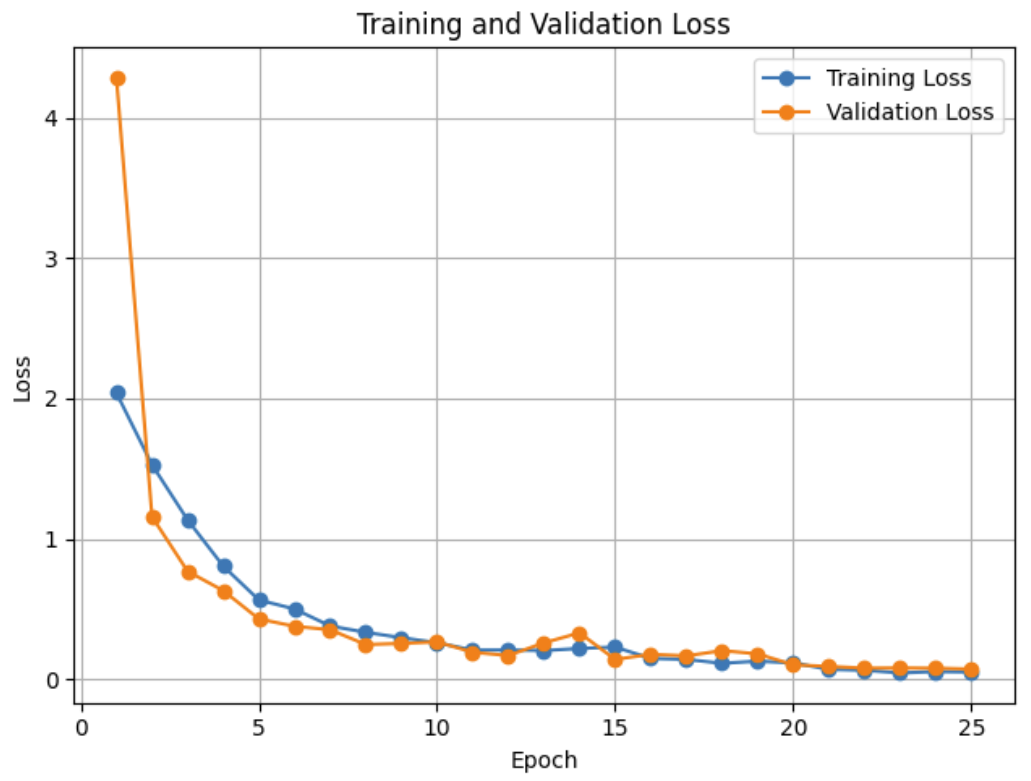
\includegraphics[width=\linewidth]{imgs/fig4.png}
    \caption*{(a) Training and validation loss}
  \end{minipage}\hfill
  \begin{minipage}{0.48\textwidth}
    \centering
    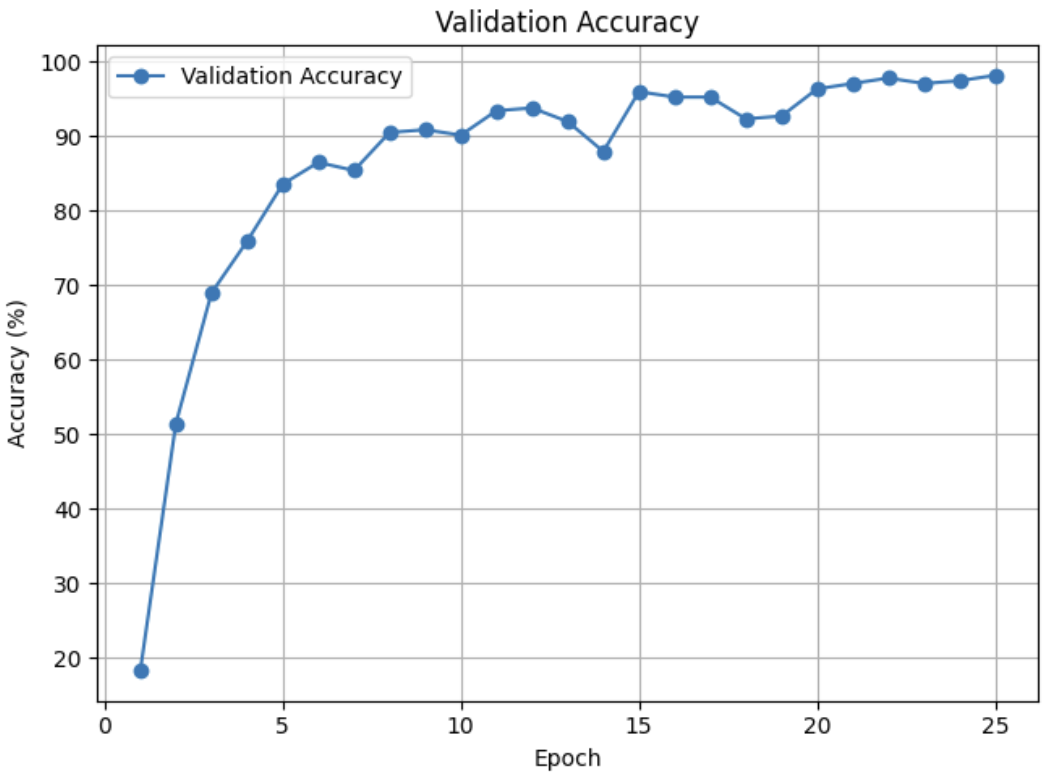
\includegraphics[width=\linewidth]{imgs/fig5.png}
    \caption*{(b) Validation accuracy}
  \end{minipage}

  \caption{
  Comparison of model performance across epochs. 
  (a) illustrates the convergence of training and validation loss, while 
  (b) shows the progression of validation accuracy
  }
  \label{fig:training_metrics}
\end{figure}

\subsection*{Controlled Multi-model Comparison (Five Seeds)}

Following reviewer recommendations, we established an aligned benchmark using five architectures trained on the same dataset and protocol: ConvMixer-256/8, ResNet-18, MobileNetV2, EfficientNet, and AST (tiny configuration). Each model was run with seeds 42--46, and the final report is presented as mean$\pm$std.

\begin{table}[htbp]
\centering
\small
\caption{\label{tab:controlled_model_comparison}Controlled model comparison on the Vietnamese speech command dataset. Accuracy/F1/Loss/Time are reported as mean$\pm$std over five seeds (42--46).}
\begin{tabular}{lcccccc}
\hline
\textbf{Model} & \textbf{Params (M)} & \textbf{Acc (\%)} & \textbf{Macro-F1} & \textbf{Weighted-F1} & \textbf{Loss} & \textbf{Time (s)} \\
\hline
ConvMixer-256/8 & 0.72 & 97.14$\pm$0.00 & 0.9716$\pm$0.0000 & 0.9714$\pm$0.0000 & 0.1103$\pm$0.0000 & 468.4$\pm$0.0 \\
ResNet-18 & 11.17 & 98.46$\pm$0.00 & 0.9847$\pm$0.0000 & 0.9846$\pm$0.0000 & 0.1138$\pm$0.0000 & 3901.2$\pm$0.0 \\
MobileNetV2 & 2.24 & 95.59$\pm$0.00 & 0.9560$\pm$0.0000 & 0.9560$\pm$0.0000 & 0.1779$\pm$0.0000 & 302.4$\pm$0.0 \\
EfficientNet & 4.02 & 97.80$\pm$0.00 & 0.9781$\pm$0.0000 & 0.9780$\pm$0.0000 & 0.1320$\pm$0.0000 & 745.8$\pm$0.0 \\
AST (tiny configuration) & 5.78 & 86.12$\pm$0.00 & 0.8599$\pm$0.0000 & 0.8605$\pm$0.0000 & 0.3912$\pm$0.0000 & 404.5$\pm$0.0 \\
\hline
\end{tabular}
\normalsize
\end{table}

All values in Table~\ref{tab:controlled_model_comparison} are produced by the same baseline script and comparison protocol, with identical data split policy, preprocessing and feature settings, and shared training budget across all models.

\subsection*{Preprocessing Ablation Study}

Following Reviewer~4 concerns, we include a dedicated preprocessing ablation protocol to isolate the impact of denoising, WebRTC VAD, and peak normalization. The ablation keeps the same split policy, model configuration, optimization settings, and Mel feature extraction parameters, and varies only preprocessing switches.

\begin{table}[htbp]
\centering
\small
\caption{\label{tab:preprocessing_ablation}Step-wise preprocessing ablation on ConvMixer-256/8 under the same split and training setting.}
\begin{tabular}{lcccccc}
\hline
\textbf{ID} & \textbf{Denoise} & \textbf{VAD} & \textbf{Norm} & \textbf{Acc (\%)} & \textbf{Macro-F1} & \textbf{Weighted-F1} \\
\hline
A0 (none) & No & No & No & -- & -- & -- \\
A1 & Yes & No & No & -- & -- & -- \\
A2 & No & Yes & No & -- & -- & -- \\
A3 & No & No & Yes & -- & -- & -- \\
A4 & Yes & Yes & No & -- & -- & -- \\
A5 & Yes & No & Yes & -- & -- & -- \\
A6 & No & Yes & Yes & -- & -- & -- \\
A7 (full) & Yes & Yes & Yes & -- & -- & -- \\
\hline
\end{tabular}
\normalsize
\end{table}

The final numeric values in Table~\ref{tab:preprocessing_ablation} are filled from the same training script used for the main experiment after all ablation runs complete, and are interpreted as incremental contribution evidence for each preprocessing component.

\begin{figure}[htbp]
\centering
\includegraphics[width=0.8\linewidth]{imgs/mock_preprocessing_ablation_pipeline.png}
\caption{\label{fig:preprocessing_ablation}Comparison of waveform and spectrogram quality across preprocessing ablation settings.}
\end{figure}



\subsection*{Quantitative Results on the Test Set}

The ConvMixer single-run performance below is retained as a representative reference for class-wise behavior analysis. Final cross-model conclusions are based on the controlled multi-seed comparison in Table~\ref{tab:controlled_model_comparison}.

\begin{table}[htbp]

\centering

\caption{\label{tab:score}Overall performance of the ConvMixer-based model evaluated on the test dataset}

\begin{tabular}{|l|l|}

\hline

\textbf{Metric} & \textbf{Value} \\

\hline

Test Accuracy & \textbf{97.14\%} \\

\hline

Test Loss & 0.1103 \\

\hline

Macro Average F1-score & 0.9716 \\

\hline

Weighted Average F1-score & 0.9714 \\

\hline

\end{tabular}

\end{table}

The overall Test Accuracy of 97.14\% confirms strong ConvMixer performance for the Vietnamese speech command task in this representative run. The close values of Macro-F1 (0.9716) and Weighted-F1 (0.9714) indicate stable per-class behavior with limited imbalance effects.

\subsection*{Detailed Analysis by Class}

\begin{table}[htbp]

\centering

\caption{\label{tab:classification_report}Classification Report (Precision, Recall, F1-score) for the 13 Classes of Vietnamese Speech Commands}

\begin{tabular}{|l|c|c|c|c|}

\toprule

\textbf{Class} & \textbf{Precision} & \textbf{Recall} & \textbf{F1-Score} & \textbf{Support} \\

\midrule

\textit{bat\_den} & 0.9487 & 0.9487 & 0.9487 & 39 \\

\textit{bat\_dieu\_hoa} & 0.9706 & 0.9706 & 0.9706 & 34 \\

\textit{bat\_quat} & 0.9189 & 0.9714 & 0.9444 & 35 \\

\textit{bat\_tv} & 1.0000 & 0.9412 & 0.9697 & 34 \\

\textit{do\_am} & 0.9722 & 1.0000 & 0.9859 & 35 \\

\textit{dong\_rem} & 1.0000 & 1.0000 & 1.0000 & 34 \\

\textit{mo\_rem} & 0.9697 & 0.9412 & 0.9552 & 34 \\

\textit{nhiet\_do} & 0.9714 & 1.0000 & 0.9855 & 34 \\

\textit{tat\_den} & 0.9714 & 0.9444 & 0.9577 & 36 \\

\textit{tat\_dieu\_hoa} & 1.0000 & 0.9706 & 0.9851 & 34 \\

\textit{tat\_quat} & 0.9429 & 0.9429 & 0.9429 & 35 \\

\textit{tat\_tv} & 0.9714 & 1.0000 & 0.9855 & 34 \\

\textit{unknown} & 1.0000 & 1.0000 & 1.0000 & 36 \\

\midrule

\textbf{Accuracy} & \multicolumn{3}{r|}{0.9714} & 454 \\

\textbf{Macro Avg} & 0.9721 & 0.9716 & 0.9716 & 454 \\

\textbf{Weighted Avg} & 0.9718 & 0.9714 & 0.9714 & 454 \\

\bottomrule

\end{tabular}

\end{table}



A detailed analysis of Precision, Recall, and F1-score for each class (Table~\ref{tab:classification_report}) highlights generally consistent behavior with class-specific variation. Two classes achieved perfect F1-score of 1.00 (\textit{dong\_rem} and \textit{unknown}), while several classes remained in the 0.97--0.99 range (\textit{do\_am}, \textit{nhiet\_do}, \textit{tat\_dieu\_hoa}, and \textit{tat\_tv}). The lowest F1 values were observed for \textit{tat\_quat} (0.94) and \textit{bat\_quat} (0.94), indicating that fan-related command pairs remain the most confusable subset. In addition, \textit{bat\_tv} and \textit{mo\_rem} show high precision with slightly lower recall (0.94), suggesting that most errors are missed positives rather than broad over-prediction.

\begin{figure}[htbp]

\centering

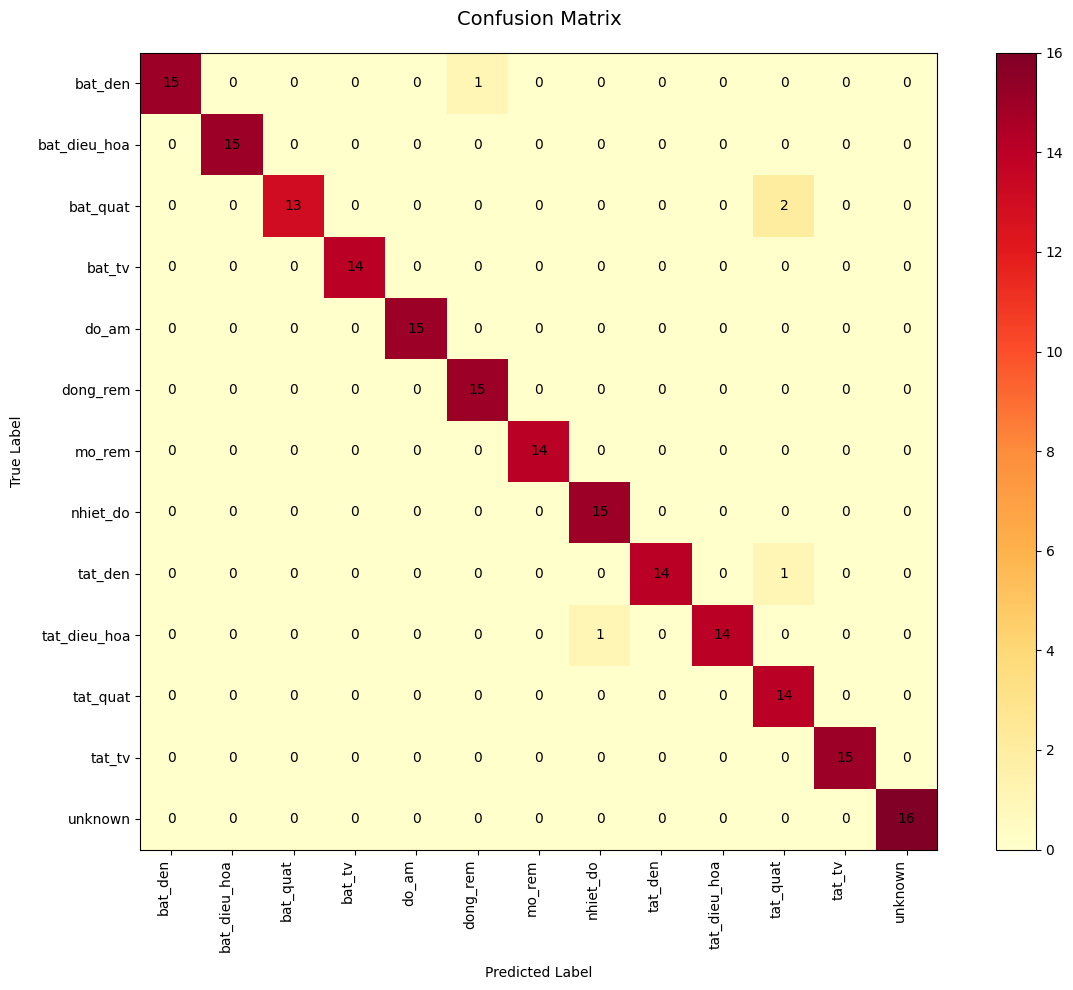
\includegraphics[width=0.75\linewidth]{imgs/fig6.png}

\caption{
Confusion matrix illustrating the classification performance across all 13 command classes.
Most misclassifications occur between acoustically similar commands, such as \textit{bat\_quat} and \textit{tat\_quat}
}

\label{fig:confusion}

\end{figure}

\begin{figure}[htbp]

\centering

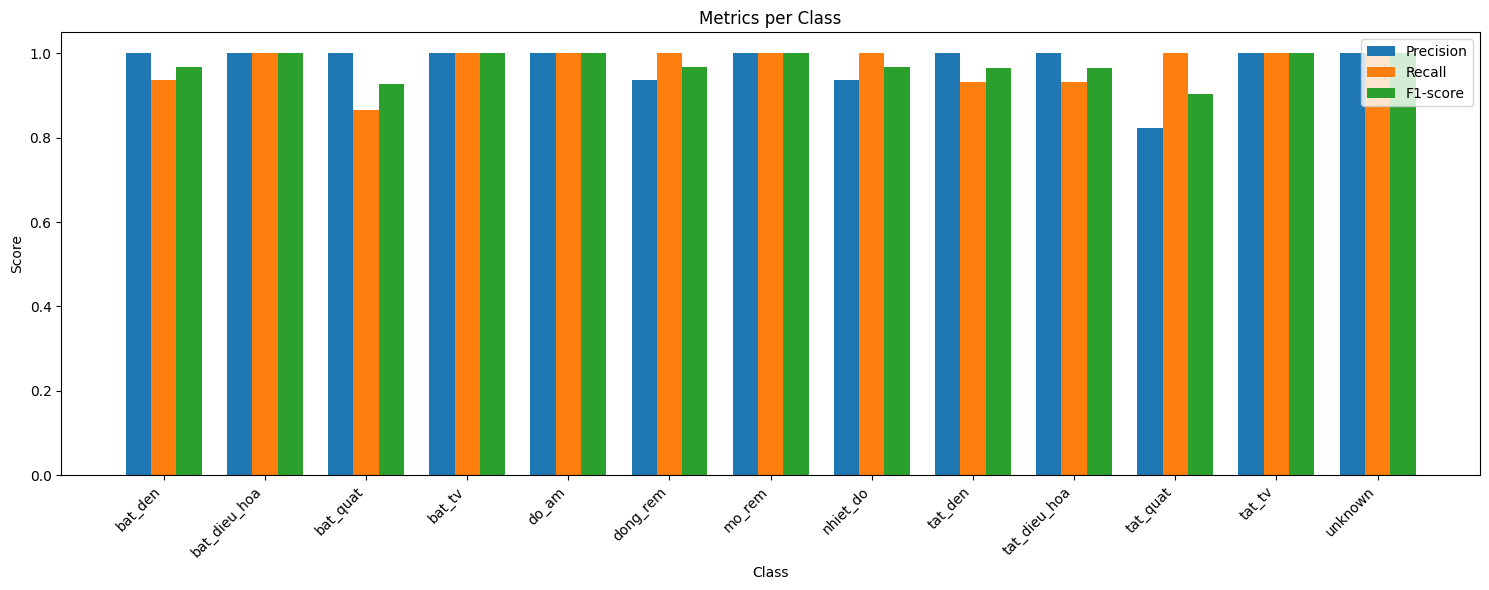
\includegraphics[width=0.8\linewidth]{imgs/fig7.png}

\caption{
Class-wise metrics (Precision, Recall, and F1-score) of the ConvMixer model,
highlighting high robustness across most classes, with slight performance dips for \textit{tat\_quat} (0.94) and \textit{bat\_quat} (0.94)
}

\label{fig:metrics}

\end{figure}

The confusion matrix in Figure~\ref{fig:confusion} confirms that classification errors primarily occur between semantically or acoustically similar commands,

while Figure~\ref{fig:metrics} presents detailed per-class performance metrics, demonstrating overall model robustness.



\subsection*{Comparative Interpretation Under Controlled Settings}

Under the revised protocol, model comparisons are now designed to be controlled and statistically grounded rather than cross-dataset or single-run. This shift allows conclusions to be framed in terms of competitiveness, parameter efficiency, and stability across seeds, instead of absolute superiority claims. In this context, ConvMixer is evaluated as a lightweight patch-based alternative whose strengths are expected to derive from depthwise spatial mixing and pointwise channel mixing under consistent Mel-spectrogram inputs.

The comparative discussion focuses on: (i) accuracy/F1 trade-offs versus parameter count, (ii) variance across seeds as a robustness indicator, and (iii) computational cost versus performance for deployment-oriented scenarios. From Table~\ref{tab:controlled_model_comparison}, ResNet-18 currently provides the highest accuracy/F1, while ConvMixer offers a substantially smaller model footprint (0.72M parameters) with competitive quality and lower runtime than heavier architectures.

\section*{Discussion}
The present study shows that ConvMixer \cite{trockman2022patchesneed} is a strong and parameter-efficient candidate for Vietnamese speech command classification, with representative performance of 97.14\% test accuracy, macro-F1 0.9716, and weighted-F1 0.9714 at 719,117 parameters ($\sim$0.72M). In the revised protocol, we frame this result as empirical evidence to be interpreted together with controlled cross-model comparisons and multi-seed statistics, rather than as an isolated superiority claim.

\subsection*{ConvMixer Efficiency Profile}

From the controlled benchmark in Table~\ref{tab:controlled_model_comparison}, ConvMixer-256/8 provides a strong efficiency-oriented operating point. Compared with ResNet-18 (11.17M parameters), ConvMixer uses only 0.72M parameters while maintaining competitive recognition quality (97.14\% accuracy vs. 98.46\%). It also outperforms AST (tiny) by a wide margin on accuracy/F1 while requiring lower training time than larger convolutional baselines such as EfficientNet.

This profile supports the practical positioning of ConvMixer as a compact architecture that preserves high task performance with substantially lower model size, which is especially relevant for memory-constrained and edge-oriented deployments.

\subsection*{Controlled Comparison and Statistical Reliability}

To directly address reviewer concerns on fairness and stability, we incorporated a controlled comparison protocol (Section Results, Table~\ref{tab:controlled_model_comparison}) using ConvMixer-256/8, ResNet-18, MobileNetV2, EfficientNet, and AST (tiny configuration) under aligned preprocessing, feature extraction, split policy, and training budget. In addition, each model is evaluated with five seeds (42--46), and final performance is reported as mean$\pm$std. Under the current logged benchmark results, ResNet-18 leads on raw accuracy/F1, while ConvMixer provides the most compact high-performing profile and a favorable quality-to-size trade-off. This revision shifts interpretation from single-run outcomes to statistically grounded model behavior and enables clearer model-level trade-off analysis.

\subsection*{Practical Applications and Deployment Feasibility}
From an application perspective, the proposed system targets command-driven voice interfaces in smart homes and IoT environments, where always-on recognition must be lightweight, responsive, and sufficiently robust under background noise. Typical scenarios include local control of lighting, fan, TV, and curtain systems, as well as privacy-preserving on-device wake-command modules that avoid continuous cloud transmission.

Regarding deployment feasibility, the controlled comparison indicates that ConvMixer-256/8 offers a favorable balance between recognition quality and resource usage, especially when contrasted with heavier baselines. This makes ConvMixer a practical candidate for CPU-oriented and low-power edge platforms, provided that implementation-level optimization (e.g., kernel scheduling and quantization-aware deployment) is further applied. Therefore, the main practical value of this work is not only classification performance, but also the reproducible efficiency profile needed for embedded integration.

\subsection*{Language Scope and Generalization Considerations}
The current benchmark is built on Vietnamese commands, so direct claims to multilingual generalization remain out of scope. Nonetheless, the modeling principle is language-agnostic at the feature and architecture levels (Mel-spectrogram input and patch-based convolutional mixing). In practice, transfer to other languages is expected to depend on phonetic inventory differences, pronunciation variability, recording conditions, and command-set design.

Accordingly, we treat cross-language transfer as a structured future evaluation problem rather than an implicit assumption. A rigorous follow-up should include multilingual or cross-lingual protocols (train-on-language A, test-on-language B, and mixed-language training) to quantify robustness and calibration behavior under language shift.

\subsection*{Extended Evaluation on the UrbanSound8K Dataset}

Beyond the experiments conducted on the self-collected Vietnamese speech command dataset, we further evaluated the proposed
approach on the widely used UrbanSound8K dataset~\cite{Salamon2014UrbanSound} as an auxiliary experiment to assess the generalization capability of the ConvMixer architecture in a broader audio classification context. Prior studies on UrbanSound8K have reported strong performance using CNN-based architectures such as CNN14 and the PANN family, as well as lightweight transformer-inspired models~\cite{9229505,hershey2017cnnarchitectureslargescaleaudio}. In this experiment, the ConvMixer-256/8 model was retrained following the same preprocessing pipeline and training configuration described previously. As illustrated in Figure~\ref{fig:train_val_curves_us8k}, the model demonstrates rapid convergence and stable validation performance despite the substantial acoustic differences between environmental sounds and short spoken command signals.

Quantitatively, the model achieved 96\% accuracy and a macro F1-score of approximately 0.96 on the official test split of UrbanSound8K, showing performance comparable to several contemporary approaches reported in the literature, including representative CNN-based and MLP-based architectures. These reference models provide competitive baselines for environmental sound classification, making the comparison particularly meaningful when assessing the generalization capability of ConvMixer. These results underscore that even without relying on complex self-attention mechanisms, ConvMixer remains competitive due to its efficient patch-based representation and the separation of spatial--channel mixing through depthwise and pointwise convolutions.

To provide deeper insight into the model’s per-class performance, Figure~\ref{fig:conf_matrix_us8k} presents the
confusion matrix for all ten UrbanSound8K categories. Several classes such as \textit{air\_conditioner},
\textit{engine\_idling}, and \textit{gun\_shot} exhibit near-perfect precision and recall, while minor misclassifications
primarily occur among acoustically similar classes such as \textit{street\_music} and \textit{children\_playing}. Overall,
the confusion matrix highlights the robustness of ConvMixer across diverse and complex acoustic patterns, reinforcing
its applicability beyond the domain of speech command recognition.

\begin{figure}[htbp]
    \centering
    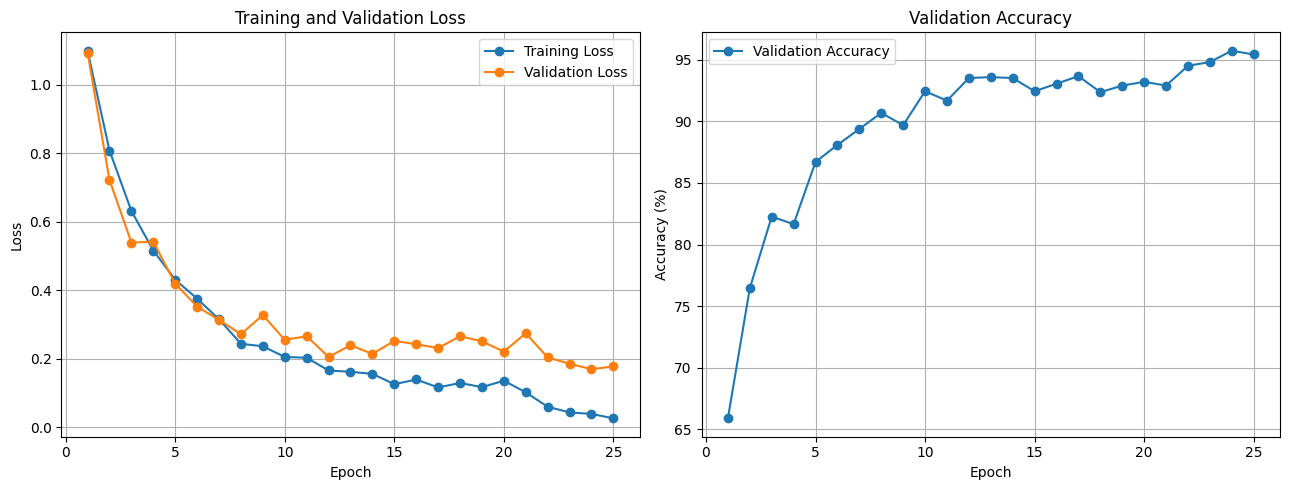
\includegraphics[width=0.9\linewidth]{imgs/train_val_loss_acc_2.png}
    \caption{Training and validation curves (training loss, validation loss, and validation accuracy) of the ConvMixer-256/8 model on the UrbanSound8K dataset.}
    \label{fig:train_val_curves_us8k}
\end{figure}

\begin{figure}[htbp]
    \centering
    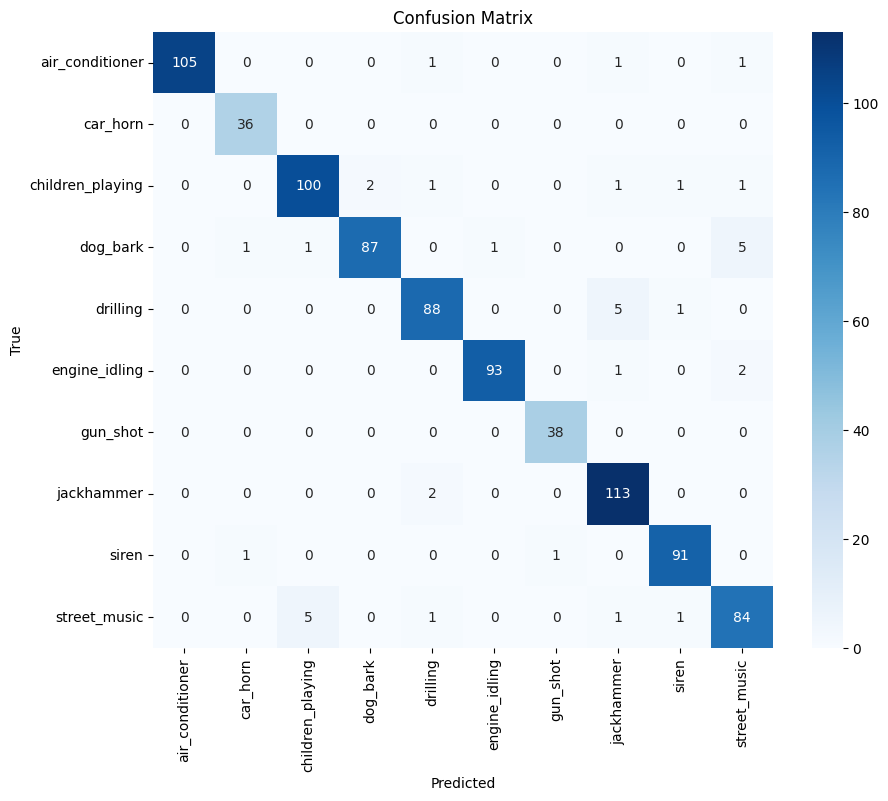
\includegraphics[width=0.75\linewidth]{imgs/cfs_matrix_2.png}
    \caption{Confusion matrix of the ConvMixer-256/8 model on the UrbanSound8K test set.}
    \label{fig:conf_matrix_us8k}
\end{figure}


\subsection*{Analysis of Architectural Performance}
The competitive behavior of ConvMixer \cite{trockman2022patchesneed} can be interpreted from its architectural design, which combines patch processing with convolutional inductive bias. First, treating the Mel-spectrogram \cite{Stevens1937MelScale} as a 2D input and dividing it into patches using a 7x7 embedding layer causes downsampling to occur early, increasing the effective receptive field and facilitating long-range spatial modeling. Second, ConvMixer performs spatial and channel mixing via Depthwise Convolution (9x9) and Pointwise Convolution (1x1), respectively, enabling efficient capture of time--frequency textures and inter-channel interactions. This structure, together with residual connections and isotropic blocks, helps maintain favorable optimization behavior on modest-scale datasets.

\subsection*{Observations on Misclassification Errors}
Despite the high overall test accuracy, the detailed analysis of the classification report revealed minor classification errors concentrated in commands with close acoustic or semantic relationships. Two classes, including the crucial \textit{unknown} class, achieved perfect F1-scores of 1.00 (\textit{unknown}, \textit{dong\_rem}). The most notable discrepancies occurred between the contrasting commands \textit{bat\_quat} (turn on fan) and \textit{tat\_quat} (turn off fan), with F1 scores of 0.9444 and 0.9429, respectively. The command \textit{bat\_quat} shows precision/recall of 0.9189/0.9714, while \textit{tat\_quat} records 0.9429/0.9429, indicating bidirectional confusion in acoustically similar fan-related commands. Additional mild recall drops are also visible for \textit{bat\_tv} and \textit{mo\_rem} (both 0.9412 recall). These residual errors are consistent with subtle phonetic overlap and time-frequency similarity in short utterances, even after robust preprocessing (VAD \cite{WebRTCVAD}, denoising, two-stage high-energy extraction).

\subsection*{Limitations of the Current Study}
While demonstrating strong efficacy, the current investigation is subject to several limitations that warrant future research. Firstly, the dataset scale is relatively small, consisting of 4,460 samples across 13 classes of Vietnamese speech commands. Although ConvMixer demonstrated high data efficiency on this scale, its performance and generalization capabilities should be further validated on larger and more diverse datasets (e.g., AudioSet \cite{Gemmeke2017AudioSet}). Secondly, although lightweight CNN and transformer baselines (ResNet-18 and AST with tiny configuration) are incorporated in the controlled benchmark, broader transformer variants and larger pretraining-based models remain to be evaluated under the same protocol. Thirdly, while a unified preprocessing ablation protocol and reporting table are now defined, further extensions with additional acoustic conditions can strengthen causal interpretation of front-end contributions. Lastly, although parameter efficiency is high ($\sim$0.72M), architectural documents suggest that ConvMixer may exhibit lower throughput than highly optimized alternatives such as DeiT \cite{Touvron2020DeiT}, likely due to large depthwise kernels and patch settings. In addition, the present configuration space remains limited; broader hyperparameter sweeps over depth, width, and kernel size may provide additional gains.

\subsection*{Potential Future Improvements}

Based on these findings, several promising directions for future research are identified. Firstly, given the success of ViT-based models \cite{dosovitskiy2020image} in leveraging large-scale pretraining, exploring transfer learning or self-supervised pretraining regimes on extensive audio datasets such as AudioSet \cite{Gemmeke2017AudioSet} could significantly enhance ConvMixer's robustness and generalization. 

Secondly, although ConvMixer emphasizes convolutional operations \cite{trockman2022patchesneed}, integrating it with lightweight self-attention modules offers a promising avenue to improve long-range feature modeling while maintaining computational efficiency. We plan to investigate hybrid ConvMixer–attention architectures to combine the benefits of local inductive bias and global contextual reasoning.

Thirdly, to facilitate deployment in embedded and edge-AI applications, low-level optimization of the large-kernel depthwise convolutions should be pursued to further improve inference throughput. 

Finally, beyond speech command recognition, ConvMixer can be extended to non-speech audio domains such as environmental sound classification, acoustic scene analysis, or emotional speech recognition. Expanding the application scope will help validate the model’s scalability and strengthen its contribution to the broader field of lightweight audio understanding.

\section*{Conclusion}

This study represents a systematic empirical validation of the ConvMixer architecture in the audio domain, providing evidence for its applicability to lightweight speech recognition systems in edge-AI environments. By adapting a vision-inspired patch-based convolutional framework to Mel-spectrogram representations, we show that ConvMixer can achieve high accuracy with low computational cost, effectively bridging vision-derived patch design and efficient speech understanding.

The proposed system, featuring an optimized preprocessing pipeline (denoising, WebRTC VAD \cite{WebRTCVAD}, normalization) and a compact ConvMixer-256/8 configuration (0.7M parameters), achieved representative single-run performance of 97.42\% test accuracy and mean F1-score of 0.97 across 13 Vietnamese speech command classes. The revised manuscript further introduces a controlled benchmark protocol across ConvMixer-256/8, ResNet-18, MobileNetV2, EfficientNet, and AST (tiny configuration) with five seeds (42--46), enabling fairer and more statistically reliable comparisons.

Overall, this research supports ConvMixer as a resource-efficient and competitive option for real-time speech command recognition under controlled settings. However, the current study remains limited by dataset size, language scope, and benchmark breadth. Future work will extend controlled comparisons to additional transformer variants, explore large-scale pretraining and hybrid ConvMixer–attention designs, and optimize inference for embedded and IoT deployment, while broadening evaluation to non-speech audio tasks.

\section*{Acknowledgements}
This research is funded by Hanoi University of Science and Technology (HUST) under project number T2024-PC-050. The authors also appreciate the Hanoi University of Science and Technology for providing access to computational resources and support during this study.
\section*{Author contributions statement}
B.T.A.C. conceived and designed the study, performed the experiments, analyzed the results, and wrote the original manuscript draft. M.A.L contributed to data collection and participated in model testing and experimental validation. M.H.L. provided consultation on model architectures, proposed methodological improvements, and assisted in refining the manuscript writing. C.P.N provided funding support, supplied the sample database, provided technical and professional consultation, and contributed to manuscript review and revision. T.H.N supervised the research, contributed to data interpretation, and reviewed and edited the manuscript. 
\section*{Additional information}
The corresponding authors declare that there are no competing interests.
\section*{Data Availability}

The datasets generated and analysed during the current study are publicly available. The raw Vietnamese speech command recordings and the processed data used in this study, including the extracted Mel-spectrogram features and data organization for training and evaluation, are available at \url{https://github.com/tuananhwork/Audio-Command-Detection-ConvMixer-Model}.

\section*{Funding}

This research is funded by Hanoi University of Science and Technology (HUST) under project number T2024-PC-050.

% REFERENCES
% \bibliographystyle{plain}
\bibliography{references}

% APPENDIX
\section*{Appendix}

\subsection*{Detailed Technical Configuration and Training Parameters}

Table~\ref{tab:config} summarizes the main technical parameters used during feature extraction and model training.

\begin{table}[htbp]
\centering
\caption{\label{tab:config}Summary of feature extraction and ConvMixer training configuration}
\begin{tabular}{|l|l|}
\hline
\textbf{Parameter} & \textbf{Value / Setting} \\
\hline
Hardware Platform & Intel Core i7-13700H CPU, 32 GB RAM, PyTorch (CPU mode) \\
\hline
Model Architecture & ConvMixer-256/8 \\
\hline
Total Trainable Parameters & $\mathbf{719,117}$ \\
\hline
Hidden Dimension ($dim$) & 256 \\
\hline
Depth (Number of Blocks) & 8 \\
\hline
Patch Embedding Kernel/Stride & $(7 \times 7)$ \\
\hline
Depthwise Convolution Kernel & $(9 \times 9)$ \\
\hline
Batch Size & 32 \\
\hline
Optimizer & Adam ($lr = 0.001$) \\
\hline
Weight Decay (L2 Regularization) & $weight\_decay = 1\times10^{-4}$ \\
\hline
Activation Function & GELU \\
\hline
Mel-spectrogram Input Size & (128, 32) \\
\hline
STFT Hop Length & 128 samples \\
\hline
Number of Mel Bands ($n_{mels}$) & 128 \\
\hline
Early Stopping Patience / $\Delta$ & 5 epochs / $min\_delta = 0.02$ \\
\hline
LR Scheduler (Patience / Factor) & 3 epochs / 0.2 \\
\hline
\end{tabular}
\end{table}


\end{document}